\section{Introduction}

\begin{frame}
	\frametitle{Outline}
	
	\LARGE
	
	\begin{itemize}
		\item Introduction
		\item Related Work
		\item PTracking
		\item Activity Forecasting Approach
		\item Experimental Evaluation
		\item Conclusions
	\end{itemize}
\end{frame}

\begin{frame}
	\frametitle{Problem}
	
	\begin{center}
		\begin{tikzpicture}
			\node at (0,0) [draw=white,ultra thick,inner sep=0pt]
			{
				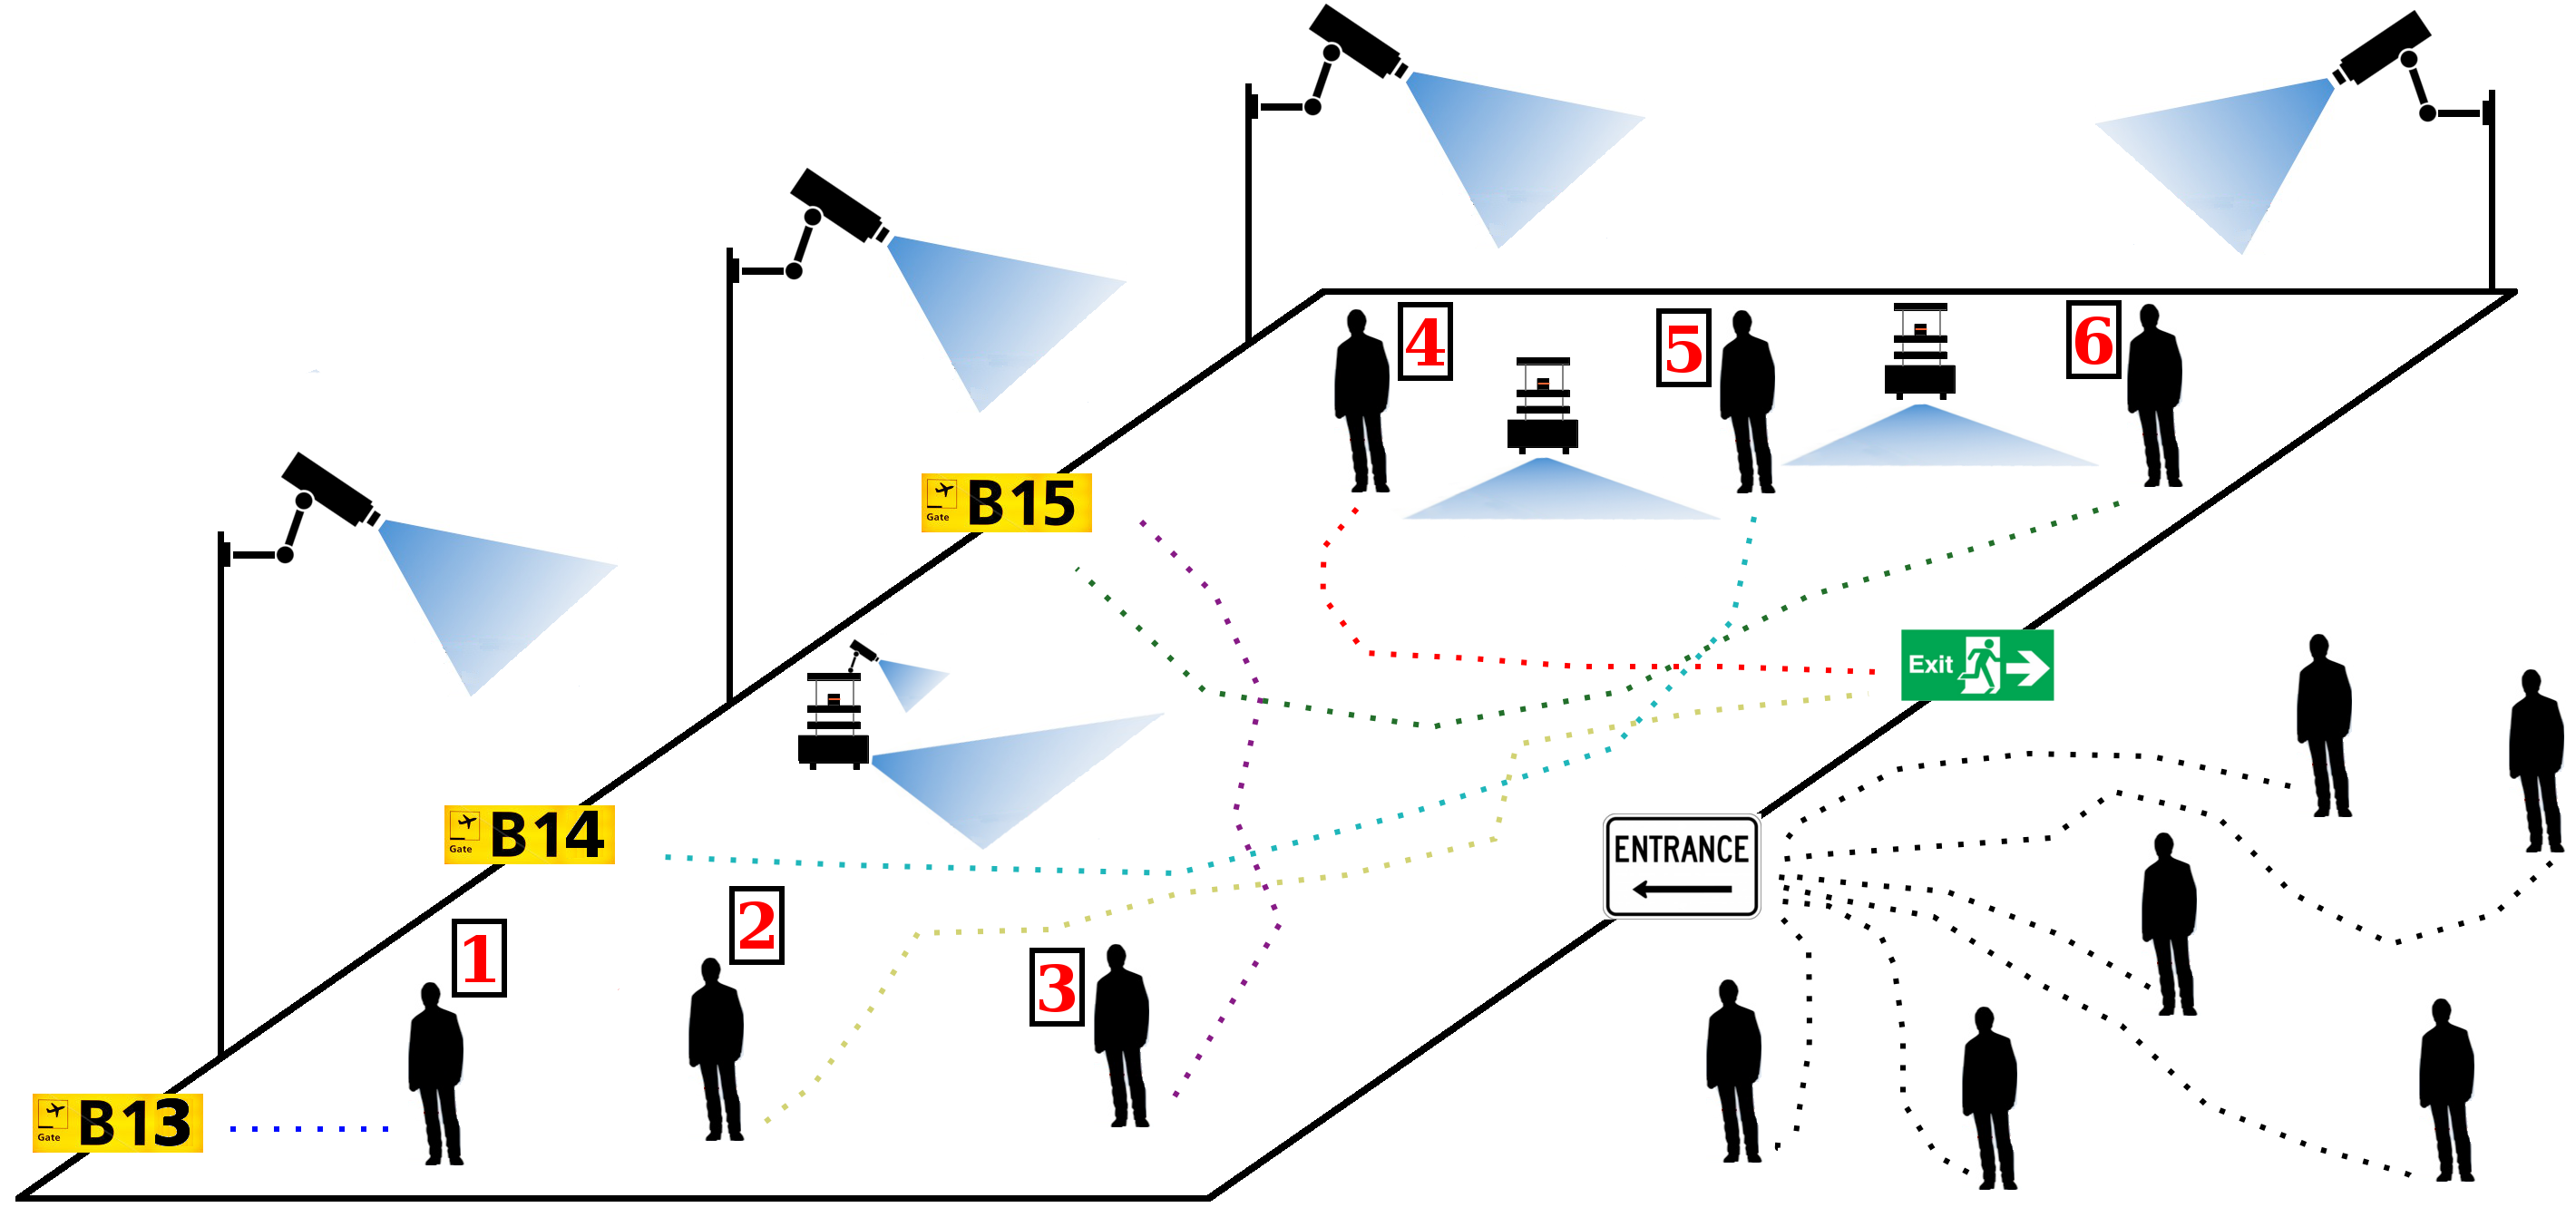
\includegraphics[width=\linewidth]{Figures/Problem.png}
			};
		\end{tikzpicture}
	\end{center}
\end{frame}

\begin{frame}
	\frametitle{Motivation}
	
	\vspace{0.2cm}
	
	\Large
	
	\begin{block}{Objective}
		\textbf{Understanding} the concept of human preference \textbf{allows} to perform higher levels
		of reasoning about future human actions. Likewise, the \textbf{knowledge} of a goal also gives
		information about \textbf{what} a person might do
	\end{block}
	
	\vspace{0.3cm}
	
	Example of application fields:
	\begin{itemize}
		\item Automatic video surveillance
		\item Human-Robot Interaction
		\item Domestic robots
	\end{itemize}
\end{frame}
